% Updated by SL (with Claude) on 4/6/26
% ---- Title ----
% ---- Section heading command (bold, all-caps, 11pt) ----
\newcommand{\sectionhead}[1]{%
  \vspace{6pt}%
  \noindent\textbf{#1}%
  \vspace{4pt}%
}
% ---- Indented block for sub-items (ALCF systems, LCRC clusters) ----
\newenvironment{indentblock}{%
  \begin{list}{}{%
    \setlength{\leftmargin}{0.3in}%
    \setlength{\rightmargin}{0pt}%
    \setlength{\itemsep}{6pt}%
    \setlength{\parsep}{0pt}%
  }%
  \item[]%
}{%
  \end{list}%
}
\vspace{4pt}

\noindent
  \textbf{ARGONNE NATIONAL LABORATORY}

\vspace{4pt}

% ---- Section: FACILITIES ----
\sectionhead{FACILITIES}

Argonne National Laboratory has access to three main facilities for computing
resources; data and networking; and data analytics and visualization. These facilities are the Argonne
Leadership Computing Facility, The Joint Laboratory for System Evaluation, and The Laboratory
Computing Resource Center.

% ---- Subsection: ALCF ----
\sectionhead{ARGONNE LEADERSHIP COMPUTING FACILITY (ALCF)}

\begin{center}
  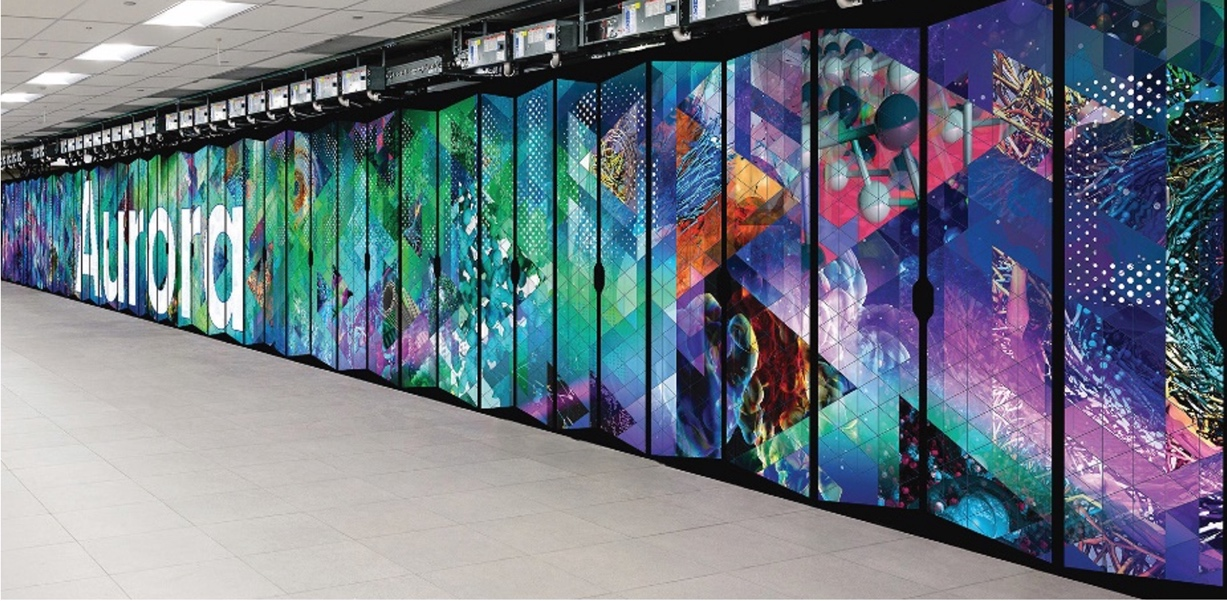
\includegraphics[width=4.5in]{../figs/image1.jpeg}
\end{center}

ALCF resources include leadership-class supercomputers, an AI testbed, advanced data storage systems,
high-performance networking capabilities, and a wide variety of software tools and services to help
facility users achieve their science goals.

\begin{indentblock}
The ALCF AI-Testbed provides an infrastructure of next-generation AI-accelerator machines. It
aims to help evaluate usability and performance of machine-learning-based high-performance
computing applications running on these accelerators. Currently, the production AI-Testbed
consists of Cerebras, SambaNova, Graphcore, and Groq systems.

Polaris, a 44-petaflop CPU/GPU hybrid resource, will allow users to prepare and scale their codes
and ultimately their science for future exascale systems. Polaris is comprised of 560 nodes with 4
NVIDIA A100 GPUs each. The system is fully integrated with the combined 200-petabyte file
systems ALCF deployed in 2020, with increased data-sharing support.

Aurora, Argonne\textquoteright s first exascale computer, features Intel\textquoteright s Data Center GPU Max Series GPUs
and Intel XEON Max Series CPUs with HBM, a CPU-GPU interconnect (PCI-e), the HPE
Slingshot fabric system interconnect, and a Cray EX platform. Aurora is fully installed and has
been transitioned to operations. Aurora\textquoteright s revolutionary architecture supports machine learning
and data science workloads alongside traditional modeling and simulation workloads.
\end{indentblock}

\noindent Aurora System Specifications

\begin{center}
  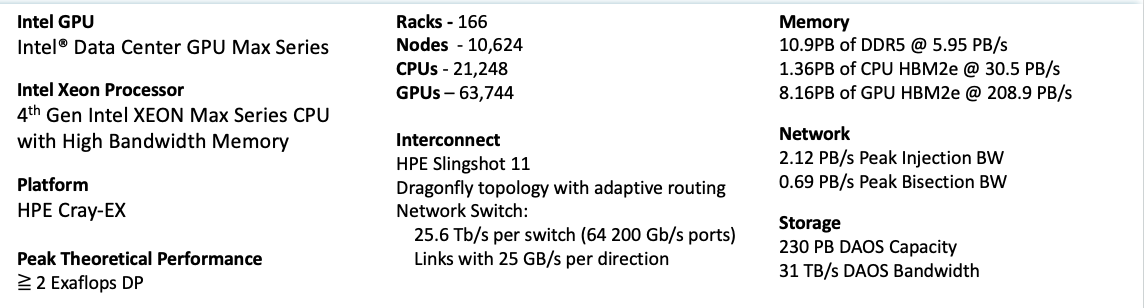
\includegraphics[width=6.35in]{../figs/image2.png}
\end{center}

Sophia is comprised of 24 NVIDIA DGX A100 nodes. Each DGX A100 node comprises eight NVIDIA
A100 Tensor Core GPUs and two AMD Rome CPUs that provide 22 nodes with 320 GB of GPU
memory and two nodes with 640 GB of GPU memory (8,320 GB in total) for training artificial
intelligence (AI) datasets, while also enabling GPU-specific and -enhanced high-performance computing
(HPC) applications for modeling and simulation. A 15-terabyte solid-state drive offers up to 25 gigabits
per second in bandwidth. Sophia has a dedicated HDR200 compute fabric wired in a fat-tree topology.

Crux is an HPE Cray EX Liquid Cooled system with a peak performance of 1.18 PF, comprised of 64
compute blades connected via Slingshot. Each blade has 4 compute nodes for a total of 256 nodes in the
system. Each compute node has dual AMD EPYC 7742 64-Core Processors. Each CPU core supports up
to two hyperthreads for a total of 256 threads possible per node. Each CPU has 128 GB of DDR4 memory
for a total of 256 GB per node.

Currently, the ALCF provides allocations on its resources based on competitive proposals through the
Innovative and Novel Computational Impact on Theory and Experiment (INCITE) program, the ASCR
Leadership Computing Challenge (ALCC), and the ALCF Director\textquoteright s Discretionary (DD) Program.
Allocations for the Early Science Program (ESP) come from preproduction time or Director\textquoteright s
Discretionary time. Historically, specialized programs in production come from discretionary (DD).

% ---- Subsection: JLSE ----
\sectionhead{THE JOINT LABORATORY FOR SYSTEM EVALUATION (JLSE)}

The Joint Laboratory for System Evaluation (JLSE) is a collaboration between the Mathematics and
Computer Science (MCS) Division and the Argonne Leadership Computing Facility (ALCF) with the aim
of evaluating future high-performance computing platforms, developing system software, and measuring
power/energy. JLSE hosts more than two dozen different cutting-edge hardware platforms, including Intel
development GPU cards (code names XeHP and DG1), as well as NVIDIA A100 and RTX8000 cards.
The post-Moore architecture lab in MCS, which is part of JLSE, hosts an FPGA testbed.

% ---- Subsection: LCRC ----
\sectionhead{LABORATORY COMPUTING RESOURCE CENTER (LCRC)}

Apart from the ALCF facilities, Argonne also hosts several other resources in the Laboratory Computing
Resource Center (LCRC).

\begin{indentblock}
Improv, our newest cluster, has 825 dual-socket compute nodes with AMD 7713 64-core
processors (2.0 GHz) (or 128 cores per node) and 256 GB DDR4 memory. 68 nodes have 4TB
NVMe SSD, and 12 of those have 1024 GB DDR4, instead of 256 GB. The high-performance
interconnect is Nvidia/Mellanox HDR200 (14 core, 35 edge switches). There are 12 HDR200
connections to LCRC\textquoteright s existing data storage system so you will have access to all the same files
between LCRC clusters.

Swing, our GPU cluster, has 6 public compute nodes and 8 NVIDIA A100 GPUS per node, 1-2TB DDR4 and 320-640GB GPU memory per node, and 128 CPU cores per compute node with
an InfiniBand HDR Interconnect.

Bebop, the oldest computing cluster in LCRC, has 664 public nodes, with 128 GB of memory on
each node.
\end{indentblock}

% ---- Subsection: CELS GCE ----
\sectionhead{CELS GENERAL COMPUTING ENVIRONMENT (GCE)}

The CELS Systems Team operates the General Computing Environment (GCE) to support the research of
CELS scientists and their collaborators. The GCE includes a collection of systems including Linux login
and compute nodes including various GPU nodes, macOS compute nodes, interactive Windows nodes,
and macOS and Linux desktop nodes. It also includes project-specific dedicated compute nodes and
storage.

GCE data storage resources include 2PB of NFS-based shared file storage, 4PB of S3 compatible object
storage, and offers Globus-based file transfers into and out of GCE as well as into and out of Box Cloud
Storage.

GCE is connected to the Argonne networking backbone via redundant 100GbE links to redundant edge
routers.

% ---- Subsection: RPL ----
\sectionhead{RAPID PROTOTYPING LABORATORY (RPL)}

Argonne National Laboratory is a leader in Autonomous Discovery (AD). Preparing laboratories to
implement AD experimental strategies and integrate automated instrumentation requires an immense
effort that includes experimental design, instrument integration, workflow development, and
troubleshooting. The Rapid Prototyping Laboratory (RPL) serves as a prototyping space for Argonne\textquoteright s
AD effort and is a vibrant software and robotics hub where scientists collaborate, train the next-generation
workforce, drive innovation, and foster an open-source environment. The RPL develops robotics software
at all levels --- from low-level instrument drivers to high-level application programming interfaces
(APIs). Key challenges include repurposing traditional lab spaces to incorporate robotic systems;
developing open-source interfaces that allow different systems to interact and seamlessly perform
scientific workflows; and designing systems that are flexible enough to combine different elements in
new ways as an experiment progresses.

\begin{center}
  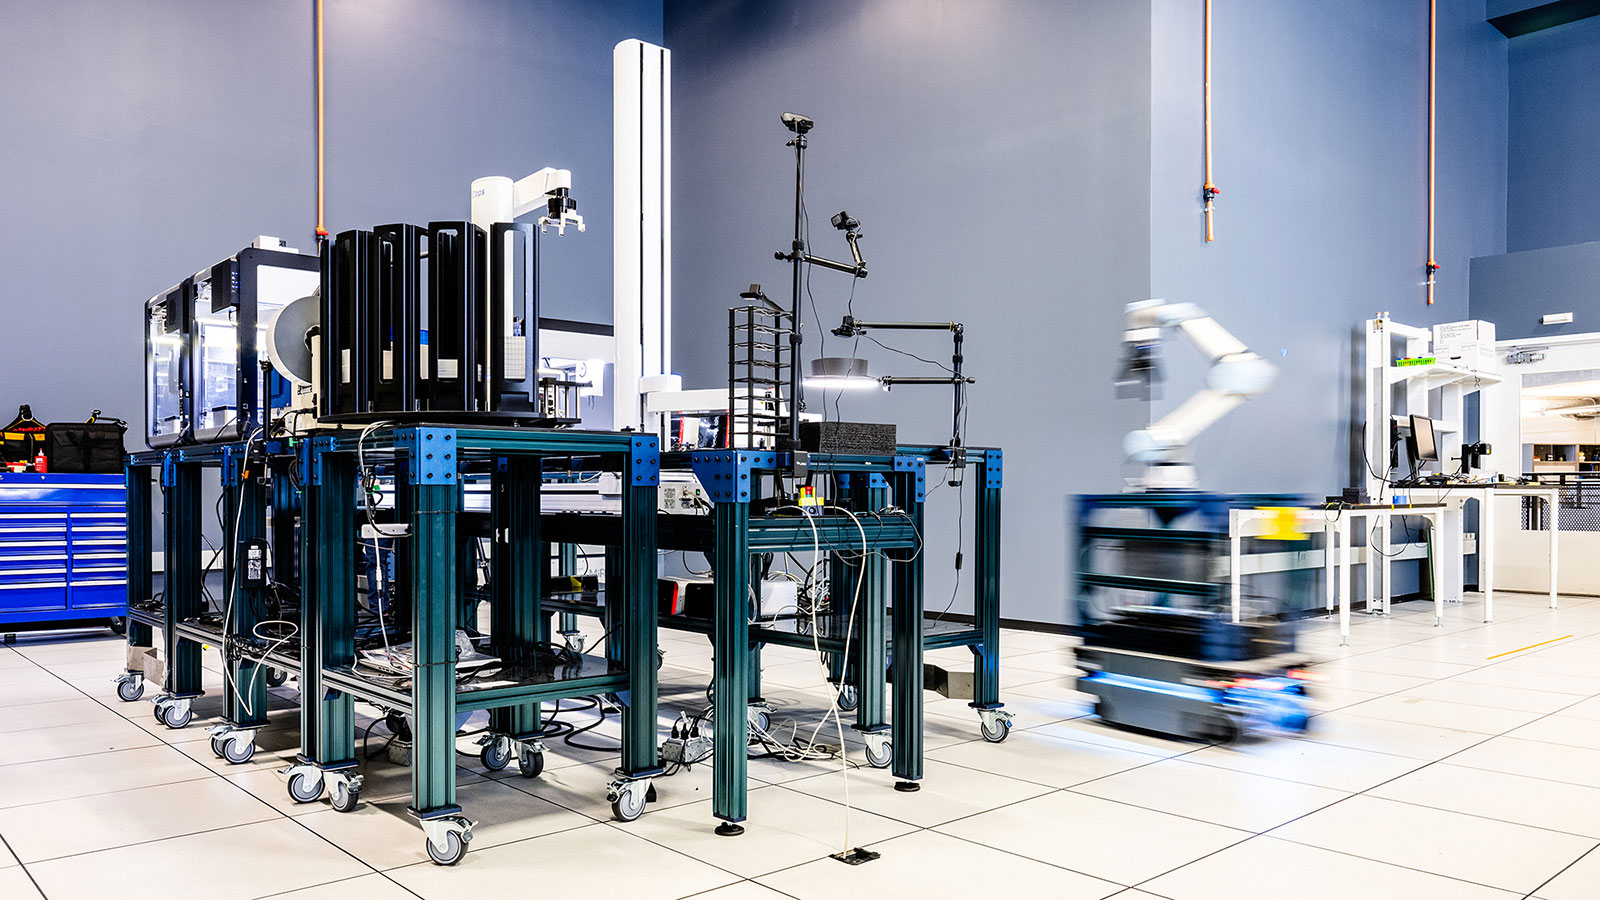
\includegraphics[width=4.50in]{../figs/image3.jpeg}
\end{center}

The RPL currently contains a functioning robotic Workcell composed of a variety of laboratory
automation robots, including three Opentrons OT-2 liquid handling robots, a Hudson SciClops Microplate
Handler, a Brooks PreciseFlex 400 (PF400) robotic arm for sample movement and several other
instruments (see Figure above). Software advancements made by the RPL in the creation of this Workcell
have been successfully applied to the implementation of several other automated experimentation
platforms across the Argonne campus with applications including biology, electrochemistry, and quantum
sensing. One instance is tailored for molecular biology and microbiology applications and contains liquid
handling robots, a plate reader, an incubator rack, a microplate sealer, a microplate peeler, as well as
several other instruments necessary for the implementation of a standard set of biological protocols. The
efficacy of this autonomous laboratory has been demonstrated in the discovery of novel peptides with
anti-microbial properties.
